\documentclass[11pt]{report}

\usepackage{graphicx}
\usepackage{framed}

\marginparwidth 0.5in 
\oddsidemargin 0.25in 
\evensidemargin 0.25in 
\marginparsep 0.25in
\topmargin 0.0in 
\textwidth 6in \textheight 8.5in

\title{HW2: Individual Contribution}
\author{bolt1003}

\begin{document}
\maketitle

\chapter{Application Domain Specification}

\subsection{User Profile Management (bolt1003)}
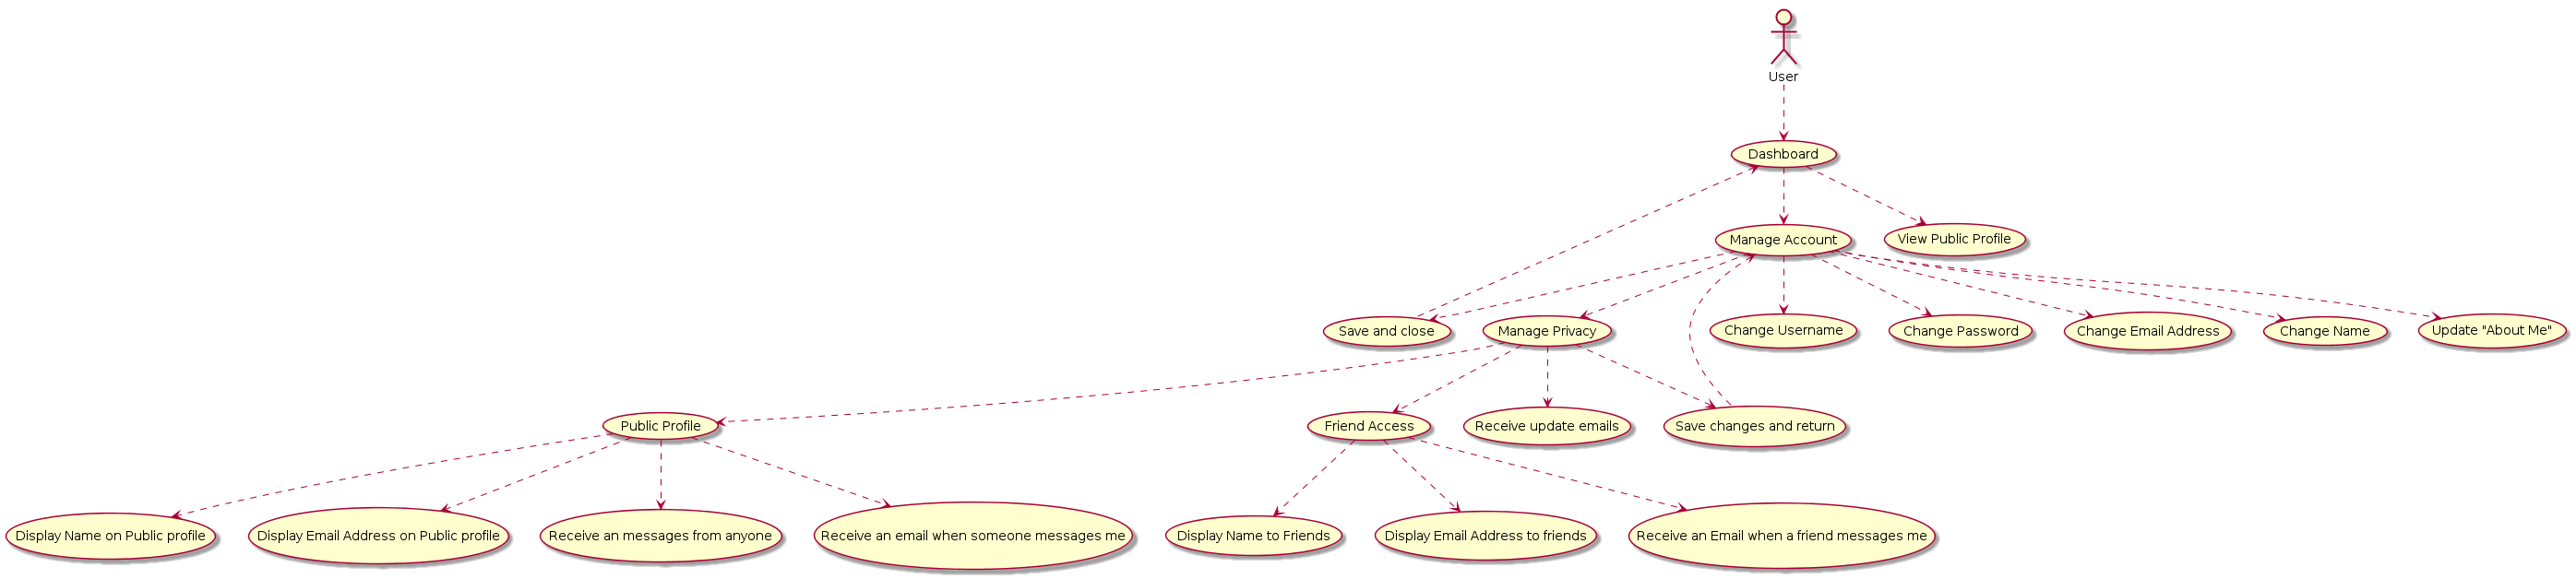
\includegraphics[width=\textwidth]{diagrams/bolt1003}

\section{Use Case Descriptions}

\subsection{Create Project from main menu(bolt1003)}
\begin{tabular}{ p{2cm} p{12cm} }
 \hline
 \\
 \textit{Actors:} & Users of sQuire. \\ 
 \\
 \textit{Goals:} & Create a Project. \\
 \\
 \textit{Pre-conditions:} & The user is logged in and at the bashboard. \\
 \\
 \textit{Summary:} & The user creates a project. \\ 
 \\
 \textit{Related use cases:} & None. \\ 
 \\
 \textit{Steps:} & \begin{enumerate}
  \item User selects the "+" icon and a wizard appears.
  \item A name is choosen for the project.
  \item Language is selected from a drop down menu.
  \item User clicks finish.
 \end{enumerate} \\
 \\
 \textit{Alternatives:} & Create project from the editor. \\
 \\
 \textit{Post-conditions:} & The user assigns permissions to access the project. \\
 \\
\hline
\end{tabular}

\subsection{Open a project (bolt1003)}
\begin{tabular}{ p{2cm} p{12cm} }
 \hline
 \\
 \textit{Actors:} & Users of sQuire. \\ 
 \\
 \textit{Goals:} & Choose the desired project and open it. \\
 \\
 \textit{Pre-conditions:} & One or more projects are available, the user is logged in and at the dashboard. \\
 \\
 \textit{Summary:} & User looks through a list of projects and selects the desired project. \\ 
 \\
 \textit{Related use cases:} & None. \\ 
 \\
 \textit{Steps:} & \begin{enumerate}
  \item User clicks on projects in the menu bar.
  \item A list of projects appears and the user clicks on the desired project.
 \end{enumerate} \\
 \\
 \textit{Alternatives:} & Open a project from recent projects. \\
 \\
 \textit{Post-conditions:} & User closes sQuire. \\
 \\
\hline
\end{tabular}

\subsection{View User Profile(bolt1003)}
\begin{tabular}{ p{2cm} p{12cm} }
 \hline
 \\
 \textit{Actors:} & Users of sQuire. \\ 
 \\
 \textit{Goals:} & Users views their public profile page. \\
 \\
 \textit{Pre-conditions:} & \begin{enumerate}
  \item The user has registered for an account.
  \item The user is logged in.
  \item The user is at the dashboard.
 \end{enumerate} \\
 \\
 \textit{Summary:} & User opens their profile to see the public view of the profile.\\ 
 \\
 \textit{Related use cases:} & User modifies their profile. \\ 
 \\
 \textit{Steps:} & \begin{enumerate}
  \item The user selects their avatar.
  \item A drop down appears and the user selects "View public profile".
 \end{enumerate} \\
 \\
 \textit{Alternatives:} & None \\
 \\
 \textit{Post-conditions:} & None. \\
 \\
\hline
\end{tabular}

\subsection{Modify User Profile(bolt1003)}
\begin{tabular}{ p{2cm} p{12cm} }
 \hline
 \\
 \textit{Actors:} & Users of sQuire. \\ 
 \\
 \textit{Goals:} & Users updates their profile. \\
 \\
 \textit{Pre-conditions:} & \begin{enumerate}
  \item The user has registered for an account.
  \item The user is logged in.
  \item The user is at the dashboard.
 \end{enumerate} \\
 \\
 \textit{Summary:} & User navigates to their profile to change their username.\\ 
 \\
 \textit{Related use cases:} & The user modifies their email address or biography. \\ 
 \\
 \textit{Steps:} & \begin{enumerate}
  \item The user select their avatar.
  \item A drop down appears and the users selects "My profile".
  \item The user selects modify. 
  \item The user changes their username.
  \item The user clicks update to save the changes.
  \item The user clicks finish to disable modify.
 \end{enumerate} \\
 \\
 \textit{Alternatives:} & \begin{enumerate} 
  \item Step 4: The user changes their password.
  \item Step 4: The user changes their email.
  \item Step 4: The user changes their "About Me" information.
  \item Step 4: The user changes their name.
 \end{enumerate} \\
 \\
 \textit{Post-conditions:} & The user returns to the dashboard or exits sQuire. \\
 \\
\hline
\end{tabular}

\subsection{Modify notifications from friends (bolt1003)}
\begin{tabular}{ p{2cm} p{12cm} }
 \hline
 \\
 \textit{Actors:} & Users of sQuire. \\ 
 \\
 \textit{Goals:} & Users modifies email updates from friends. \\
 \\
 \textit{Pre-conditions:} & \begin{enumerate}
  \item The user has registered for an account.
  \item The user is logged in.
  \item The user is at the dashboard.
 \end{enumerate} \\
 \\
 \textit{Summary:} & User navigates to the privacy manager and changes notifications options for people in their friends list.\\ 
 \\
 \textit{Related use cases:} & The user modifies global freind permissions. \\ 
 \\
 \textit{Steps:} & \begin{enumerate}
  \item The user select their avatar.
  \item A drop down appears and the users selects "My profile".
  \item The users selects manage privacy.
  \item The user selects friend communication management.
  \item The user selects a friend.
  \item The user click the toggle switch next to "Receive email updates when this friends messages me".
 \end{enumerate} \\
 \\
 \textit{Alternatives:} & \begin{enumerate} 
  \item Step 5: The user clicks the toggle switch next to "Display email address to this friend".
  \item Step 5: The user clicks the toggle switch next to "Display name to this friend".
 \end{enumerate} \\
 \\
 \textit{Post-conditions:} & The user returns to the dashboard or exits sQuire. \\
 \\
\hline
\end{tabular}

\subsection{Modify public messaging preferences (bolt1003)}
\begin{tabular}{ p{2cm} p{12cm} }
 \hline
 \\
 \textit{Actors:} & Users of sQuire. \\ 
 \\
 \textit{Goals:} & Users modifies settings to allow messages from any user on squire. \\
 \\
 \textit{Pre-conditions:} & \begin{enumerate}
  \item The user has registered for an account.
  \item The user is logged in.
  \item The user is at the dashboard.
 \end{enumerate} \\
 \\
 \textit{Summary:} & User navigates to the privacy manager and changes messaging public messaging options.\\ 
 \\
 \textit{Related use cases:} & The user changes public notifications preferences. \\ 
 \\
 \textit{Steps:} & \begin{enumerate}
  \item The user select their avatar.
  \item A drop down appears and the users selects "My profile".
  \item The users selects manage privacy.
  \item The user selects manage public privacy settings.
  \item The user click the toggle switch next to "Allow messages from any sQuire user".
 \end{enumerate} \\
 \\
 \textit{Alternatives:} & \begin{enumerate} 
  \item Step 5: The user clicks the toggle switch next to "Display email address to the public".
  \item Step 5: The user clicks the toggle switch next to "Display name to the public".
 \end{enumerate} \\
 \\
 \textit{Post-conditions:} & The user returns to the dashboard or exits sQuire. \\
 \\
\hline
\end{tabular}

\subsection{Modify global email settings (bolt1003)}
\begin{tabular}{ p{2cm} p{12cm} }
 \hline
 \\
 \textit{Actors:} & Users of sQuire. \\ 
 \\
 \textit{Goals:} & Users modifies settings to allow email notifications. \\
 \\
 \textit{Pre-conditions:} & \begin{enumerate}
  \item The user has registered for an account.
  \item The user is logged in.
  \item The user is at the dashboard.
 \end{enumerate} \\
 \\
 \textit{Summary:} & User navigates to the privacy manager and changes email preferences.\\ 
 \\
 \textit{Related use cases:} & Change public or freind notifications. \\ 
 \\
 \textit{Steps:} & \begin{enumerate}
  \item The user select their avatar.
  \item A drop down appears and the users selects "My profile".
  \item The users selects manage privacy.
  \item The user clicks the toggle switch next to "Allow email notifications".
 \end{enumerate} \\
 \\
 \textit{Alternatives:} & None. \\
 \\
 \textit{Post-conditions:} & The user returns to the dashboard or exits sQuire. \\
 \\
\hline
\end{tabular}
\end{document}